
\subsection{简介}

模拟退火是一种随机化算法。当一个问题的方案数量极大(甚至是无穷的)而且不是一个单峰函数时,我们常使用模拟退火求解。

\hr

\subsection{实现}

根据  爬山算法  的过程,我们发现:对于一个当前最优解附近的非最优解,爬山算法直接舍去了这个解。而很多情况下,我们需要去接受这个非最优解从而跳出这个局部最优解,即为模拟退火算法。

\begin{QUOTE}{}{}
\textbf{什么是退火?}(选自百度百科)
退火是一种金属热处理工艺,指的是将金属缓慢加热到一定温度,保持足够时间,然后以适宜速度冷却。目的是降低硬度,改善切削加工性;消除残余应力,稳定尺寸,减少变形与裂纹倾向;细化晶粒,调整组织,消除组织缺陷。准确的说,退火是一种对材料的热处理工艺,包括金属材料、非金属材料。而且新材料的退火目的也与传统金属退火存在异同。
\end{QUOTE}

由于退火的规律引入了更多随机因素,那么我们得到最优解的概率会大大增加。于是我们可以去模拟这个过程,将目标函数作为能量函数。

\subsubsection{模拟退火算法描述}

先用一句话概括:如果新状态的解更优则修改答案,否则以一定概率接受新状态。

我们定义当前温度为 $T$,新状态与已知状态(由已知状态通过随机的方式得到)之间的能量(值)差为 $\Delta E$($\Delta E\geqslant 0$),则发生状态转移(修改最优解)的概率为

$$
P(\Delta E)=
\begin{cases}
1&\text{新状态更优}\\
e^\frac{-\Delta E}{T}&\text{新状态更劣}
\end{cases}
$$

\textbf{注意}:我们有时为了使得到的解更有质量,会在模拟退火结束后,以当前温度在得到的解附近多次随机状态,尝试得到更优的解(其过程与模拟退火相似)。

\subsubsection{如何退火(降温)?}

模拟退火时我们有三个参数:初始温度 $T_0$,降温系数 $d$,终止温度 $T_k$。其中 $T_0$ 是一个比较大的数,$d$ 是一个非常接近 $1$ 但是小于 $1$ 的数,$T_k$ 是一个接近 $0$ 的正数。

首先让温度 $T=T_0$,然后按照上述步骤进行一次转移尝试,再让 $T=d\cdot T$。当 $T<T_k$ 时模拟退火过程结束,当前最优解即为最终的最优解。

引用一张 \href{https://en.wikipedia.org/wiki/Simulated_annealing}{Wiki - Simulated annealing} 的图片(随着温度的降低,跳跃越来越不随机,最优解也越来越稳定)。


\begin{figure}[htbp]
\centering
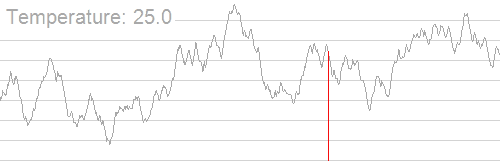
\includegraphics[width=0.7\textwidth]{docs/misc/images/a-0.png} 
\caption{注:pdf 中动图效果不好,请到 \href{https://oi-wiki.org/misc/simulated-annealing/}{网站}上浏览获得最佳效果}
\end{figure}

\hr

\subsection{代码}

此处代码以 \href{https://www.lydsy.com/JudgeOnline/problem.php?id=3680}{「BZOJ 3680」吊打 XXX}(求 $n$ 个点的带权类费马点)为例。

\begin{cppcode}
#include <cmath>
#include <cstdio>
#include <cstdlib>
#include <ctime>

const int N = 10005;
int n, x[N], y[N], w[N];
double ansx, ansy, dis;

double Rand() { return (double)rand() / RAND_MAX; }
double calc(double xx, double yy) {
  double res = 0;
  for (int i = 1; i <= n; ++i) {
    double dx = x[i] - xx, dy = y[i] - yy;
    res += sqrt(dx * dx + dy * dy) * w[i];
  }
  if (res < dis) dis = res, ansx = xx, ansy = yy;
  return res;
}
void simulateAnneal() {
  double t = 100000;
  double nowx = ansx, nowy = ansy;
  while (t > 0.001) {
    double nxtx = nowx + t * (Rand() * 2 - 1);
    double nxty = nowy + t * (Rand() * 2 - 1);
    double delta = calc(nxtx, nxty) - calc(nowx, nowy);
    if (exp(-delta / t) > Rand()) nowx = nxtx, nowy = nxty;
    t *= 0.97;
  }
  for (int i = 1; i <= 1000; ++i) {
    double nxtx = ansx + t * (Rand() * 2 - 1);
    double nxty = ansy + t * (Rand() * 2 - 1);
    calc(nxtx, nxty);
  }
}
int main() {
  srand(time(0));
  scanf("%d", &n);
  for (int i = 1; i <= n; ++i) {
    scanf("%d%d%d", &x[i], &y[i], &w[i]);
    ansx += x[i], ansy += y[i];
  }
  ansx /= n, ansy /= n, dis = calc(ansx, ansy);
  simulateAnneal();
  printf("%.3lf %.3lf\n", ansx, ansy);
  return 0;
}
\end{cppcode}

\hr

\subsection{习题}

\begin{itemize}
\item \href{https://www.lydsy.com/JudgeOnline/problem.php?id=3680}{「BZOJ 3680」吊打 XXX}
\item \href{https://www.lydsy.com/JudgeOnline/problem.php?id=4852}{「JSOI 2016」炸弹攻击}
\item \href{https://www.lydsy.com/JudgeOnline/problem.php?id=2428}{「HAOI 2006」均分数据}
\end{itemize}
